\documentclass{standalone}
\usepackage{tikz}
\usepackage{subcaption}
\usetikzlibrary{arrows.meta, decorations.pathmorphing, positioning}

\tikzset{
    cg/.style={
        draw,
        circle,
        thick,
        minimum size=0.2cm, % Adjust the size of the circle
        inner sep=0,      % Remove extra padding
        append after command={
            \pgfextra{
                \draw[thick] (\tikzlastnode.south) -- (\tikzlastnode.north);
                \draw[thick] (\tikzlastnode.west) -- (\tikzlastnode.east);
            }
        }
    }
}

\begin{document}

\centering
\begin{tikzpicture}[scale=1.2]
    \begin{subfigure}[b]{0.3\textwidth}
        \centering
        \begin{tikzpicture}
            % Draw the propeller blade section (simplified airfoil shape)
            \draw[dashed] (0,0) arc (0:360:1);
            \draw[thick] (0,-0.25) -- (0,0.25) node[above] {};

            \draw[->] (-1,0) -- (0,0) node[above, midway] {$r_0$};
            \draw[dashed] (0.5,0) arc (0:360:1.5);

            \draw[->] (-1,0) -- (0.5-0.1,-0.5) node[below, midway] {$r_t$};
            \draw[->] (-0.7,0) arc (0:270:0.3) node[midway, left] {$\Omega$};

        \end{tikzpicture}
        \caption{Top-down view of a propeller blade section}
        \label{fig:topdown}
    \end{subfigure}
    \begin{subfigure}[b]{0.3\textwidth}
        \centering
        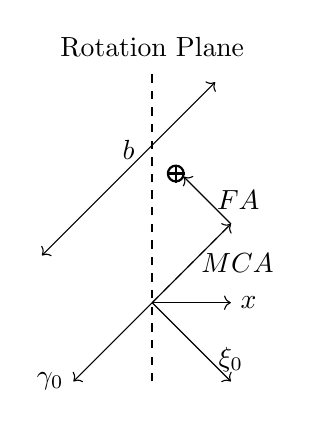
\begin{tikzpicture}
            % Some profiles look better when using plot[smooth]
        \begin{scope}[rotate=225, xshift=-2.5cm, yshift=-1cm]
            \draw[scale=3,thick=3] node[left=0.5cm] {}
                plot file{../app/foils/NACA2412.surf} -- cycle;
        \end{scope}
        % hoirzontal line
        \draw[thick, dashed] (0,-1) -- (0, 3) node[above] {Rotation Plane};
        \draw[->] (0,0) -- (1,0) node[right] {$x$};
        \draw[->] (0,0) -- (1,-1) node[above] {$\xi_0$};
        \draw[->] (0,0) -- (-1,-1) node[left] {$\gamma_0$};
        \node[cg] at (-0.75+1.05,1-0.41+1.05) {};
        \draw[dashed] (0,0) -- (1,1) node[] {};
        \draw[->] (0,0) -- (1,1) node[right, midway] {$MCA$};
        \draw[->] (1,1) -- (0.4,1.6) node[right, midway] {$FA$};

        \draw[<->] (-1-0.4,1-0.4) -- (1-0.2,3-0.2) node[above, midway] {$b$};
    \end{tikzpicture}
        \caption{Single blade section}
        \label{fig:single}
    \end{subfigure}
    \begin{subfigure}[b]{0.35\textwidth}
        \centering
        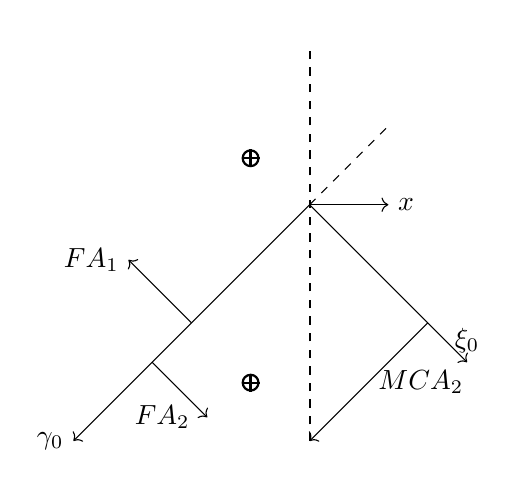
\begin{tikzpicture}
                % Some profiles look better when using plot[smooth]
            \begin{scope}[rotate=225, xshift=-1cm, yshift=-1cm]
                \draw[scale=3,thick=3] node[left=0.5cm] {}
                    plot file{../app/foils/NACA2412.surf} -- cycle;
            \end{scope}
            \begin{scope}[rotate=225, xshift=1cm, yshift=1cm]
                \draw[scale=3,thick=3] node[left=-0.5cm] {}
                    plot file{../app/foils/NACA2412.surf} -- cycle;
            \end{scope}
            % hoirzontal line
            \draw[thick, dashed] (0,-3) -- (0, 2) node[above] {};
            \draw[->] (0,0) -- (1,0) node[right] {$x$};
            \draw[->] (0,0) -- (2,-2) node[above] {$\xi_0$};
            \draw[->] (0,0) -- (-3,-3) node[left] {$\gamma_0$};
            \node[cg] at (-0.75,1-0.41) {};
            \node[cg] at (-0.75,1-0.41-3+0.15) {};
            \draw[dashed] (0,0) -- (1,1) node[] {};
            \draw[->] (-1.5,-1.5) -- (-2.5+0.2,-0.5-0.2) node[left] {$FA_1$};
            \draw[->] (-2,-2) -- (-2 + 0.5+0.2,-2.5-0.2) node[left, xshift=-0.1cm] {$FA_2$};
            \draw[->] (1.5,-1.5) -- (-1.5+1.5,-1.5-3+1.5) node[right, midway] {$MCA_2$};
        \end{tikzpicture}
        \caption{Superimposed blade sections}
        \label{fig:double}
\end{tikzpicture}

\end{document}